



%----------------------------------------------------------------------------------------

\newpage


%\section[Existing Models][Modèles existants]{Existing Models}{Modèles existants}
\section{Exploring macroscopic models of co-evolution}{Explorer les modèles macroscopiques de co-évolution}

\label{sec:macrocoevolexplo}

%----------------------------------------------------------------------------------------



\bpar{

}{
Nous proposons dans un premier temps d'introduire les modèles de co-évolution à l'échelle macroscopique en explorant les résultats produits par un modèle existant, ce qui permettra également d'introduire les méthodes et indicateurs nécessaires à l'exploration, ainsi que d'appréhender les questionnements typiques liés à ce type de modèles. En particulier, nous procédons à une exploration systématique du modèle SimpopNet~\cite{schmitt2014modelisation}, à notre connaissance l'une des rares initiatives pour modéliser la co-évolution au sein d'un système de villes.
}



%%%%%%%%%%%%%%%%%%%%%%%
\subsection{Context}{Contexte}


\bpar{
Which differences in produced knowledge can be observed, from the conceptual or thematic description of a model, to its mathematical formalisation, its implementation, its systematic exploration, up to its exploration in deep with the help of specific meta-heuristics ? Our postulate, that is a consequence of both our positioning (see \autoref{ch:positioning} on simulation) and experiments of which previously developed models are part, is that it is considerable, but furthermore of a \emph{qualitative} nature, in the sense that the nature of knowledge follows abrupt transitions during the advance of the investigation in this continuum. The SimpopNet model introduced by~\cite{schmitt2014modelisation}, which is to our knowledge the only co-evolution model in the perspective of the evolutive urban theory, is an example of such a preliminary approach that must be explored deeper, for example through systematic exploration.
}{
Un gain considérable de connaissances peut s'observer, de la description conceptuelle ou thématique d'un modèle, à sa formalisation mathématique, son implémentation, son exploration systématique, jusqu'à son exploration approfondie à l'aide de méta-heuristiques spécifiques. Notre postulat, qui découle à la fois de notre positionnement (voir le chapitre~\ref{ch:positioning} sur la simulation) et d'expériences dont les modèles déroulés précédemment font partie, est que celui-ci est important, mais surtout de nature \emph{qualitative}, c'est-à-dire que la nature même des connaissances subit des transitions abruptes lors de l'avancée de la démarche dans ce continuum.

Le modèle SimpopNet introduit par~\cite{schmitt2014modelisation}, est à notre connaissance l'unique modèle de co-évolution selon la perspective de la théorie évolutive des villes. Son comportement n'a cependant pas été exploré systématiquement, ce qui en fait un bon candidat pour notre démarche.
}


\subsubsection{Model Description}{Modèle étudié}

Nous reformulons brièvement le modèle, suivant les notations de la formulation du modèle d'interaction en~\ref{sec:interactiongibrat}, un certain nombre de paramètres et de processus se recoupant. Les villes croissent suivant une spécification qui peut être rapprochée de l'équation~\ref{eq:interactiongibrat:model}, c'est-à-dire dans ce cas spécifique
\[
\mu_i(t+1) - \mu_i (t) = \mu_i (t) \cdot \frac{\lambda^{\beta}}{N} \sum_{j} \frac{V_{ij}}{<V_{ij}>}
\]
où le potentiel est de la forme $V_{ij} = \mu_j / d_{ij}^\beta$ et $V_{ii}=0$, et $\beta$ est un paramètre de vitesse de décroissance en fonction de la distance et $\lambda$ paramètre de forme de la fonction de décroissance. Nous retrouvons ainsi notre formulation, avec $r_0 = 0$ et $w_G = \lambda^\beta \cdot N$. Comme $\lambda$ fixe la distance typique d'interaction, nous le noterons par la suite $d_G$, et $\beta$ sera noté $\gamma_G$ (il s'agit bien d'un niveau de hiérarchie en fonction de la distance).

%Le potentiel d'interaction ne dépend pas de la population de la ville d'origine, et le choix d'une fonction puissance permet de combiner un paramètre de décroissance $\lambda$ à un paramètre de forme $\beta$.

Le réseau croît à chaque pas de temps par un processus que nous pouvons qualifier de rupture de potentiel (comme décrit au chapitre~\ref{ch:thematic}) : un couple de villes est choisi, la première selon les populations avec une hiérarchie $\gamma_N$ (c'est-à-dire avec une probabilité proportionnelle à ${\mu_i}^{\gamma_N}$) et la seconde selon les forces d'interactions $\mu_i \mu_j / d_{ij}^\beta$ avec la même hiérarchie $\gamma_N$. Un lien est alors créé si le réseau n'est pas assez efficace, c'est-à-dire si $d_{ij}/d^{(N)}_{ij}> \theta_N$. Les liens créés à une date $t$ ont une vitesse $v(t)$, qui dépendra des technologies de transport courantes. La création de nouvelles intersections pour produire un graphe planaire n'est effectuée que pour les liens de vitesse semblable.

Afin d'étudier une version stylisée du modèle, nous considérons une configuration telle que $v(t > 0) = v_0$ et $v(0) = 1$ (le modèle initial considère trois valeurs de la vitesse correspondant aux réalités des technologies de transport entre 1830 et 2000).


\subsubsection{Perspectives}{Perspectives}

Mettons en perspective la structure de ce modèle. Certains choix de modélisation ne sont pas en cohérence directe avec l'application qui en est faite : par exemple, une telle précision dans la paramétrisation des dates et des vitesses (dates historiques de 1800 à 2000 et vitesse correspondant approximativement aux technologiques de transport) en fait un modèle hybride, et devrait correspondre à une application sur une configuration spatiale réelle. Dans une configuration synthétique comme employée dans le modèle, ces paramètres n'ont de sens que si l'on connait le comportement des dynamiques simulées, et en particulier le rôle de la configuration spatiale, c'est-à-dire être capable de différencier effets liés à la dynamique et effets liés à la configuration spatiale initiale. 

D'autre part, l'utilisation du modèle d'interaction sans le terme de Gibrat endogène serait difficilement adaptable pour une application du modèle sur données réelles vu les valeurs obtenues dans les études précédentes des modèles d'interaction, mais est bien cohérent dans un modèle stylisé, afin de comprendre les processus d'interaction de manière isolée, comme nous le ferons plus loin (tout en gardant à l'esprit que cette connaissance ne reflète pas nécessairement le comportement couplé, l'interaction entre les processus pouvant faire émerger de nouveaux comportements).

La formulation du potentiel, donnée ci-dessus, en $(\lambda / d_{ij})^\beta$ implique que $\lambda$ capture à la fois le poids du potentiel et la forme de la décroissance, mais contraint à une dépendance entre ces deux effets, contrairement à la spécification que nous avons utilisé précédemment. Elle ne permet par ailleurs pas d'interprétation en terme de flux limite\footnote{Le paramètre de poids dans notre modèle en~\ref{sec:interactiongibrat} donne en fait la valeur du flux lorsque l'atténuation par la distance tend vers l'infini et pour l'ensemble de la population.}.

Enfin, les règles permettant des valeurs variables de $v(t)$ et le mécanisme de non-planarité du réseau\footnote{Lorsqu'un nouveau lien est construit, celui-ci ne forme des intersections qu'avec les liens de vitesse similaire.}, permet l'introduction d'un effet tunnel, qui nous le rappellons est la non-interaction d'une infrastructure traversant un territoire avec celui-ci. L'effet est cependant exogène puisque spécifié explicitement dans les règles du modèle, contrairement au modèle d'interaction avec rétroaction des flux, dans lequel les variations de $w_N$ et $d_N$ doivent capturer un effet tunnel endogène. L'introduction d'indicateurs spécifiques pour le mesurer serait une piste intéressante de développement, mais nous nous contentons de regarder ici la hiérarchie des centralités qui en est déjà un bon indicateur\footnote{En effet, une distribution très hiérarchique des accessibilités signifie qu'il existe un petit nombre de villes très accessibles et un grand nombre peu accessibles. Si les villes importantes couvrent raisonnablement l'espace, alors leurs liens ignorent nécessairement les villes peu accessibles survolées, sinon la distribution serait moins hiérarchique.}.



%%%%%%%%%%%%%%%%%%%%%%%
\subsection{Methodology}{Méthode}

\subsubsection{Spatial configuration}{Configuration spatiale}

Un aspect important de la compréhension des processus de co-évolution impliqués dans ce modèle est le rôle de la configuration spatiale initiale dans les motifs émergents observés. Nous appliquons pour cela la méthodologie développée en~\ref{sec:computation}, permettant d'étendre l'analyse de sensibilité d'un modèle à des méta-paramètres spatiaux\footnote{Nous rappelons que dans notre cas un méta-paramètre est un paramètre permettant de générer une configuration initiale en amont du modèle.}.

\paragraph{Synthetic configuration generation}{Génération de configurations synthétiques}

Une système de villes synthétique est construit de la façon suivante (voir l'Annexe~\ref{app:sec:syntheticdata} pour la notion de données synthétiques, calibrées au premier et second ordre). Un nombre fixé de villes $N$ est réparti uniformément dans l'espace en respectant une distance minimale entre chaque, et leur population est attribuée suivant une loi rang-taille dont les paramètres $P_{m}$ et $\alpha$ peuvent être ajustés (la distribution de la taille des villes dans le modèle initial correspond à $\alpha\simeq 0.68$ avec $R^2=0.98$).

Un squelette de réseau est créé par connection progressive : l'algorithme connecte les villes deux à deux par plus proche voisin en distance euclidienne, puis itérativement sélectionne un cluster aléatoirement et le connecte perpendiculairement au lien le plus proche hors du cluster. Le réseau est ensuite étoffé par la création de raccourcis locaux, par répétitions $n_s$ fois de la sélection aléatoire d'une ville selon les populations, et sa connexion à un voisin dans un rayon $r_s$ sous conditions de degré maximal $d_s$. Le réseau final est ensuite planarisé.

Cette procédure crée des réseaux correspondant visuellement (ordre de grandeur du nombre de boucles, portée spatiale de celles-ci) à l'initialisation du modèle, sachant qu'une instance du réseau ne permet pas de déterminer les distributions de paramètres topologiques sur lesquels une calibration plus fine pourrait être opérée.



\subsubsection{Indicators}{Indicateurs}

Un aspect crucial de l'étude des modèles de simulation est la définition d'indicateurs pertinents, surtout dans le cas de modèles synthétiques où il n'est pas possible de produire des sorties directement liées aux données par exemple. Des faits stylisés très généraux, comme vouloir produire une hiérarchie urbaine ou une hiérarchie de réseau, sont relativement limités. De plus, la hiérarchie est produite mécaniquement par la majorité des modèles incluant des processus d'agrégation. Il faut donc des indicateurs plus élaborés pour comprendre les dynamiques du système. Ces indicateurs doivent notamment apporter des éléments de réponse aux questions suivantes : 
 \begin{itemize}
 	\item types de systèmes de villes produits par le modèle ;
 	\item changement dans le temps de l'organisation du système de ville ;
 	\item profils typiques de trajectoires ;
 	\item capacité à ``produire de la co-évolution''.
 \end{itemize}


Pour se concentrer sur la capacité du modèle à produire des trajectoires à la fois diverses et complexes, et par exemple sa capacité à produire des bifurcations qui se traduiraient par inversions de rang, ainsi que sa capacité à capturer différents aspects des dynamiques co-évolutives, nous proposons un jeu d'indicateurs, incluant par exemple des mesures de corrélation retardée en écho aux régimes de causalité exhibés en~\ref{sec:causalityregimes}, ou une mesure de corrélation en fonction de la distance, pour comprendre le rôle des interactions spatiales dans les couplages de trajectoires. Étant donné une variable $X_i(t)$ définie sur chacune des villes et dans le temps (qui pourra être la population ou des mesures de centralité par exemple), nous définissons les indicateurs suivants.

\begin{itemize}
  \item Indicateurs caractérisant la distribution de $X_i$ dans le temps : hiérarchie (pente de l'ajustements moindres carrés de $X_i$ en fonction du rang) $\alpha (t)$, entropie de la distribution $\varepsilon (t)$, statistiques descriptives (moyenne $\hat{\Eb{X}} (t)$ et écart-type $\hat{\sigma} (t)$).
  \item Corrélation de rang entre l'instant initial et l'instant final, qui traduit la quantité de changement dans la hiérarchie lors de l'évolution du système, et est définie par $\rho_r = \hat{\rho}\left[rg(X_i(t=0)),rg(X_i(t=t_f))\right]$, où $rg(X_i)$ est le rang de $X_i$ parmi l'ensemble des valeurs.
  \item Diversité des trajectoires $\mathcal{D}\left[X_i\right]$, qui capture une diversité de profil des séries temporelles pour la variable considérée. Avec $\tilde{X}_i(t)\in \left[0;1\right]$ les trajectoires mises à l'échelle individuellement, elle est définie par
\[
\mathcal{D}\left[X_i\right] = \frac{2}{N\cdot(N-1)}\sum_{i<j} \left(\frac{1}{T}\int_{t} \left(\tilde{X}_i(t) - \tilde{X}_j(t)\right)^2 \right)^{\frac{1}{2}}
\]
\item Changements de direction des trajectoires $\mathcal{C}\left[X_i\right]$, que nous prenons comme le nombre de points d'inflexion. Dans le cadre de ce type de modèle, qui produit majoritairement des trajectoires monotones, cet indicateur témoigne dans une certaine mesure d'une ``complexité'' des trajectoires.
\item Corrélations en fonction de la distance, pour comprendre la manière dont l'effet de la distance est traduit au niveau macroscopique. Le profil de cette fonction, au regard des valeurs des paramètres de distance d'interaction inclus dans le modèle, traduira la tendance du modèle à faire émerger tel ou tel niveau d'interaction. Elle est calculée comme
\[
\rho_d = \hat{\rho}\left[(X(\vec{x}_k,Y(\vec{x}_{k'}))\right]
\]
où $X_i, Y_i$ sont les deux variables considérées et $(k,k')$ l'ensemble des couples tels que $\norm{\vec{x}_k-\vec{x}_{k'}} - d \leq \varepsilon$ avec $\varepsilon$ seuil de tolérance (en pratique pris pour regrouper les couples par déciles de distance).
\item Corrélations retardées entre les variations des variables, pour identifier des motifs de causalité entre les variables $X$ et $Y$. Les motifs $\hat{\rho}_{\tau}$ pour l'ensemble des variables, et pour $\tau$ retard ou anticipation, sont à lire dans le sens des régimes potentiels, explorés en~\ref{sec:causalityregimes}.
\[
\rho_{\tau} = \hat{\rho}\left[\Delta X(t-\tau),\Delta Y(t)\right]
\]
\end{itemize}

% diversite : \comment[AB]{expliciter cette variance $\rightarrow$ cf methode alternative Jasss}

Ces indicateurs sont utilisés sur les variables suivantes :
\begin{itemize}
	\item populations $\mu_i(t)$,
	\item centralités de proximité
	\[c_i(t) = \frac{1}{N-1}\sum_{i\neq j} \frac{1}{d_{ij}(t)}\]
	qui capturent la position dans le système urbain,
	\item accessibilités \[X_i = \frac{1}{\sum_k \mu_k}\sum_{i\neq j} P_j \exp{\left(- d_{ij}(t)/d_G\right)}\] qui capturent l'insertion dans le système urbain.
\end{itemize}



Nous introduisons de plus divers indicateurs de topologie du réseau, pour comprendre les formes finales produites par l'heuristique : diamètre, longueur moyenne de chemin, centralité de chemin moyenne et niveau de hiérarchie, performance moyenne, longueur totale, comme ils ont été définis en~\ref{sec:staticcorrelations}.




%%%%%%%%%%%%%%%%%%%%%%%
\subsection{Results}{Résultats}


\subsubsection{Experience plan}{Plan d'expérience}

Étant donné une configuration spatiale initiale (c'est-à-dire une valeur des méta-paramètres), nous établissons le comportement des indicateurs par l'exploration d'une grille de l'espace des paramètres. Le nombre de paramètres étant restreint et l'objectif étant un premier aperçu du comportement du modèle, notamment s'il est capable de produire des dynamiques de co-évolution, nous ne faisons pas appel à des méthodes d'exploration plus élaborées. Les paramètres sont $(d_G,\gamma_G,\gamma_N,\theta_N,v_0)$ et les méta-paramètres $(N_S,\alpha_S,d_S,n_S)$. Nous prenons en compte également les méta-paramètres pour comprendre la sensibilité du modèle à l'espace.

Nous explorons une grille de 16 configurations des méta-paramètres, 324 configurations de paramètres, et 30 réplications aléatoires, ce qui correspond à $155520$ simulations. Celles-ci sont exécutées sur grille de calcul par l'intermédiaire d'OpenMole\footnote{Les résultats de simulation sont disponibles à \url{http://dx.doi.org/10.7910/DVN/RW8S36}.}.



\subsubsection{Convergence}{Convergence}


Le modèle étant stochastique, il est important de contrôler la convergence des indicateurs, qui sera plus ou moins facile selon leur variabilité. Pour quantifier la variabilité d'un indicateur $X$ par rapport à la stochasticité, nous utilisons une mesure similaire à celle de~\ref{sec:densitygeneration}, donnée par $v\left[X\right] = \hat{\mathbb{E}}\left[X\right]/\hat{\sigma}\left[X\right]$ avec les estimateurs basiques pour l'espérance et l'écart-type. Sur l'ensemble des réplications, on obtient sur l'ensemble des indicateurs donnés précédemment, une médiane pour le ratio $v\left[X\right]$ estimé au sein des réplications, estimée sur toutes les valeurs des paramètres, qui prend une valeur minimale de $3.94$, pour la moyenne de l'accessibilité à l'instant final, ce qui témoigne d'une faible variabilité stochastique. On peut de plus utiliser cette valeur pour estimer le niveau de convergence : elle correspond à un intervalle de confiance à 95\% autour de la moyenne de taille relative $0.18$ (sous hypothèse de distribution normale de la moyenne), c'est-à-dire une bonne convergence. Cet aspect est essentiel pour la robustesse des résultats.




% values of summaries for Sharpe ratios
%
%[1] "accessibilityEntropies95"
%    Min.  1st Qu.   Median     Mean  3rd Qu.     Max.     NA's 
%   4.038   13.704   35.392   95.136   93.556 4064.812        9 
%[1] "accessibilityHierarchies_alpha95"
%   Min. 1st Qu.  Median    Mean 3rd Qu.    Max.    NA's 
%  1.538   6.330   8.912   8.810  11.090  92.960       9 
%[1] "accessibilitySummaries_mean95"
%    Min.  1st Qu.   Median     Mean  3rd Qu.     Max.     NA's 
%  0.5106   2.8426   3.9498   5.2793   6.0301 155.6903        9 
%[1] "closenessEntropies95"
%   Min. 1st Qu.  Median    Mean 3rd Qu.    Max.    NA's 
%  11.25   39.70   85.78  106.72  154.51  677.88       9 
%[1] "closenessHierarchies_alpha95"
%   Min. 1st Qu.  Median    Mean 3rd Qu.    Max.    NA's 
%  2.429   5.107   6.933   7.803   9.930  48.226       9 
%[1] "closenessSummaries_mean95"
%   Min. 1st Qu.  Median    Mean 3rd Qu.    Max.    NA's 
%  1.391   3.488   5.753   6.018   7.901  39.855       9 
%[1] "populationEntropies95"
%    Min.  1st Qu.   Median     Mean  3rd Qu.     Max.     NA's 
%       3       51      953   646296    17776 35961483        9 
%[1] "populationHierarchies_alpha95"
%   Min. 1st Qu.  Median    Mean 3rd Qu.    Max.    NA's 
%      5      42     906  135579    3672 5328192       9 
%[1] "populationSummaries_mean95"
%    Min.  1st Qu.   Median     Mean  3rd Qu.     Max.     NA's 
%       1       17      382   229768     6319 11448551        9 
%[1] "complexityAccessibility"
%   Min. 1st Qu.  Median    Mean 3rd Qu.    Max.    NA's 
%     NA      NA      NA     NaN      NA      NA    2544 
%[1] "complexityCloseness"
%    Min.  1st Qu.   Median     Mean  3rd Qu.     Max.     NA's 
%  0.7363   4.6781  14.1490  16.0315  24.4733 221.7233        9 
%[1] "complexityPop"
%   Min. 1st Qu.  Median    Mean 3rd Qu.    Max.    NA's 
%     NA      NA      NA     NaN      NA      NA    2544 
%[1] "diversityAccessibility"
%    Min.  1st Qu.   Median     Mean  3rd Qu.     Max.     NA's 
%  0.6063   2.8002   6.2182   6.3092   9.0482 171.3062        9 
%[1] "diversityCloseness"
%   Min. 1st Qu.  Median    Mean 3rd Qu.    Max.    NA's 
% 0.8169  3.3100  7.3997  7.1288  9.5683 32.9526       9 
%[1] "diversityPop"
%   Min. 1st Qu.  Median    Mean 3rd Qu.    Max.    NA's 
%  1.058   4.089   7.481   8.001  10.858 115.732       9 





\subsubsection{Sensitivity to space}{Sensibilité à l'espace}

La Table~\ref{tab:macrocoevolexplo:spacematters} donne les valeurs de $\tilde{d}$ pour 16 configurations des méta-paramètres\footnote{La definition de la mesure relative de sensibilité, donnée en~\ref{sec:computation}, est pour deux diagrammes de phase $f_1,f_2$ et $d$ distance euclidienne, $\tilde{d} = 2 d(f_1,f_2)/(\Varb{f_1}+\Varb{f_2})$.}, par rapport à une configuration de référence arbitraire (première colonne). La hiérarchie au sein du système de villes initial apparaît comme le plus fort déterminant de la variabilité, puisque l'ensemble des configurations avec $\alpha_S = 1.5$ donnent des valeurs supérieures à $1.7$, ce qui témoigne d'une très forte sensibilité relative à cette hiérarchie.

Ensuite, le nombre de villes joue un rôle secondaire non négligeable, donnant les plus forts effets de l'espace. Ainsi, il est crucial de garder à l'esprit ce rôle de la configuration initiale lors de l'analyse des diagrammes de phase. Pour rester dans l'esprit du modèle initialement proposé, nous commenterons toutefois un diagramme de phase pour une configuration spatiale donnée. L'étude du modèle étendu avec intégration des méta-paramètres auxquels il est sensible comme paramètres à part entière est hors de portée de cette analyse auxiliaire.



%%%%%%%%%%%%%
\begin{table}[!ht]
\caption[Sensitivity to space of the SimpopNet model][Sensibilité à l'espace du modèle SimpopNet]{\textbf{Sensitivity to space of the SimpopNet model.}\label{tab:macrocoevolexplo:spacematters}}{\textbf{Sensibilité à l'espace du modèle SimpopNet.} Chaque colonne correspond à une instance du diagramme de phase, pour laquelle les méta-paramètres sont donnés, ainsi que la distance relative à un diagramme de référence arbitraire. En entrée on a les méta-paramètres $N_S,\alpha_S,d_S,n_S$ et en résultat des simulation la distance $\tilde{d}$.\label{tab:macrocoevolexplo:spacematters}}
\begin{tabular}{|l|l|l|l|l|l|l|l|l|l|l|l|l|l|l|l|l|}
\hline
$N_S$ & 40 & 40 & 40 & 40 & 40 & 40 & 40 & 40 & 80 & 80 & 80 & 80 & 80 & 80 & 80 & 80\\
$\alpha_S$ & 0.5 & 0.5 & 0.5 & 0.5 & 1.5 & 1.5 & 1.5 & 1.5 & 0.5 & 0.5 & 0.5 & 0.5 & 1.5 & 1.5 & 1.5 & 1.5\\
$d_S$ & 5 & 5 & 10 & 10 & 5 & 5 & 10 & 10 & 5 & 5 & 10 & 10 & 5 & 5 & 10 & 10\\
$n_S$ & 10 & 30 & 10 & 30 & 10 & 30 & 10 & 30 & 10 & 30 & 10 & 30 & 10 & 30 & 10 & 30\\\hline
$\tilde{d}$ & 0 & 0.05 & 0.26 & 0.21 & 1.79 & 1.80 & 1.79 & 1.72 & 0.44 & 0.36 & 0.42 & 0.42 & 2.25 & 2.23 & 2.24 & 2.21\\\hline
\end{tabular}
\end{table}
%%%%%%%%%%%%%



\subsubsection{Patterns}{Comportement du modèle}



La Fig.~\ref{fig:macrocoevolexplo:behavior} rend compte du comportement du modèle selon une selection parmi les divers indicateurs donnés ci-dessus. Nous commentons une configuration spatiale particulière qui correspond à un système peu hiérarchisé avec un réseau n'ayant que des raccourcis locaux, donnée par les méta-paramètres $N_S=80,\alpha_S=0.5,d_S=10,n_S=30$, qui sont les valeurs donnant des configurations les plus similaires à celle du modèle initial. Les graphes complets sont disponibles en Annexe~\ref{app:sec:macrocoevolexplo}.


Les valeurs prises par l'entropie pour les centralités (premier panel de la Fig.~\ref{fig:macrocoevolexplo:behavior}), en fonction du temps, pour $\gamma_N = 2.5$ et $v_0 = 110$, exhibent différents régimes en fonction de $d_G$ et $\gamma_G$. Une faible hiérarchie conduit à une entropie se stabilisant dans le temps, correspondant à une certaine uniformisation des distances. Au contraire, une forte hiérarchie produit un régime avec un minimum, puis une augmentation des disparités dans le temps.


Cette variété de comportements se retrouve avec la corrélation de rang $\rho_R$, que nous montrons ici pour la variable de population, en fonction de $d_G$. Celle-ci est peu sensible à $\theta_N$ et $\gamma_N$ (voir Annexe~\ref{app:sec:macrocoevolexplo}), mais varie fortement en fonction de $d_G$ et $\gamma_G$ : des interactions à plus longue distance induisent systématiquement un plus grand nombre de changements dans la hiérarchie des populations. Celles-ci peuvent avoir lieu quand la hiérarchie de la distance est faible. En résumé, l'augmentation de la portée des interactions diminuera l'inertie des trajectoires du système de villes, tandis que l'augmentation de leur hiérarchie la fera croître. Cela est relativement crédible du point de vue thématique : des interactions plus lointaines et uniformes ont plus de chances de faire changer les trajectoires individuelles.


%%%%%%%%%%%%%%%%
\begin{figure}
	%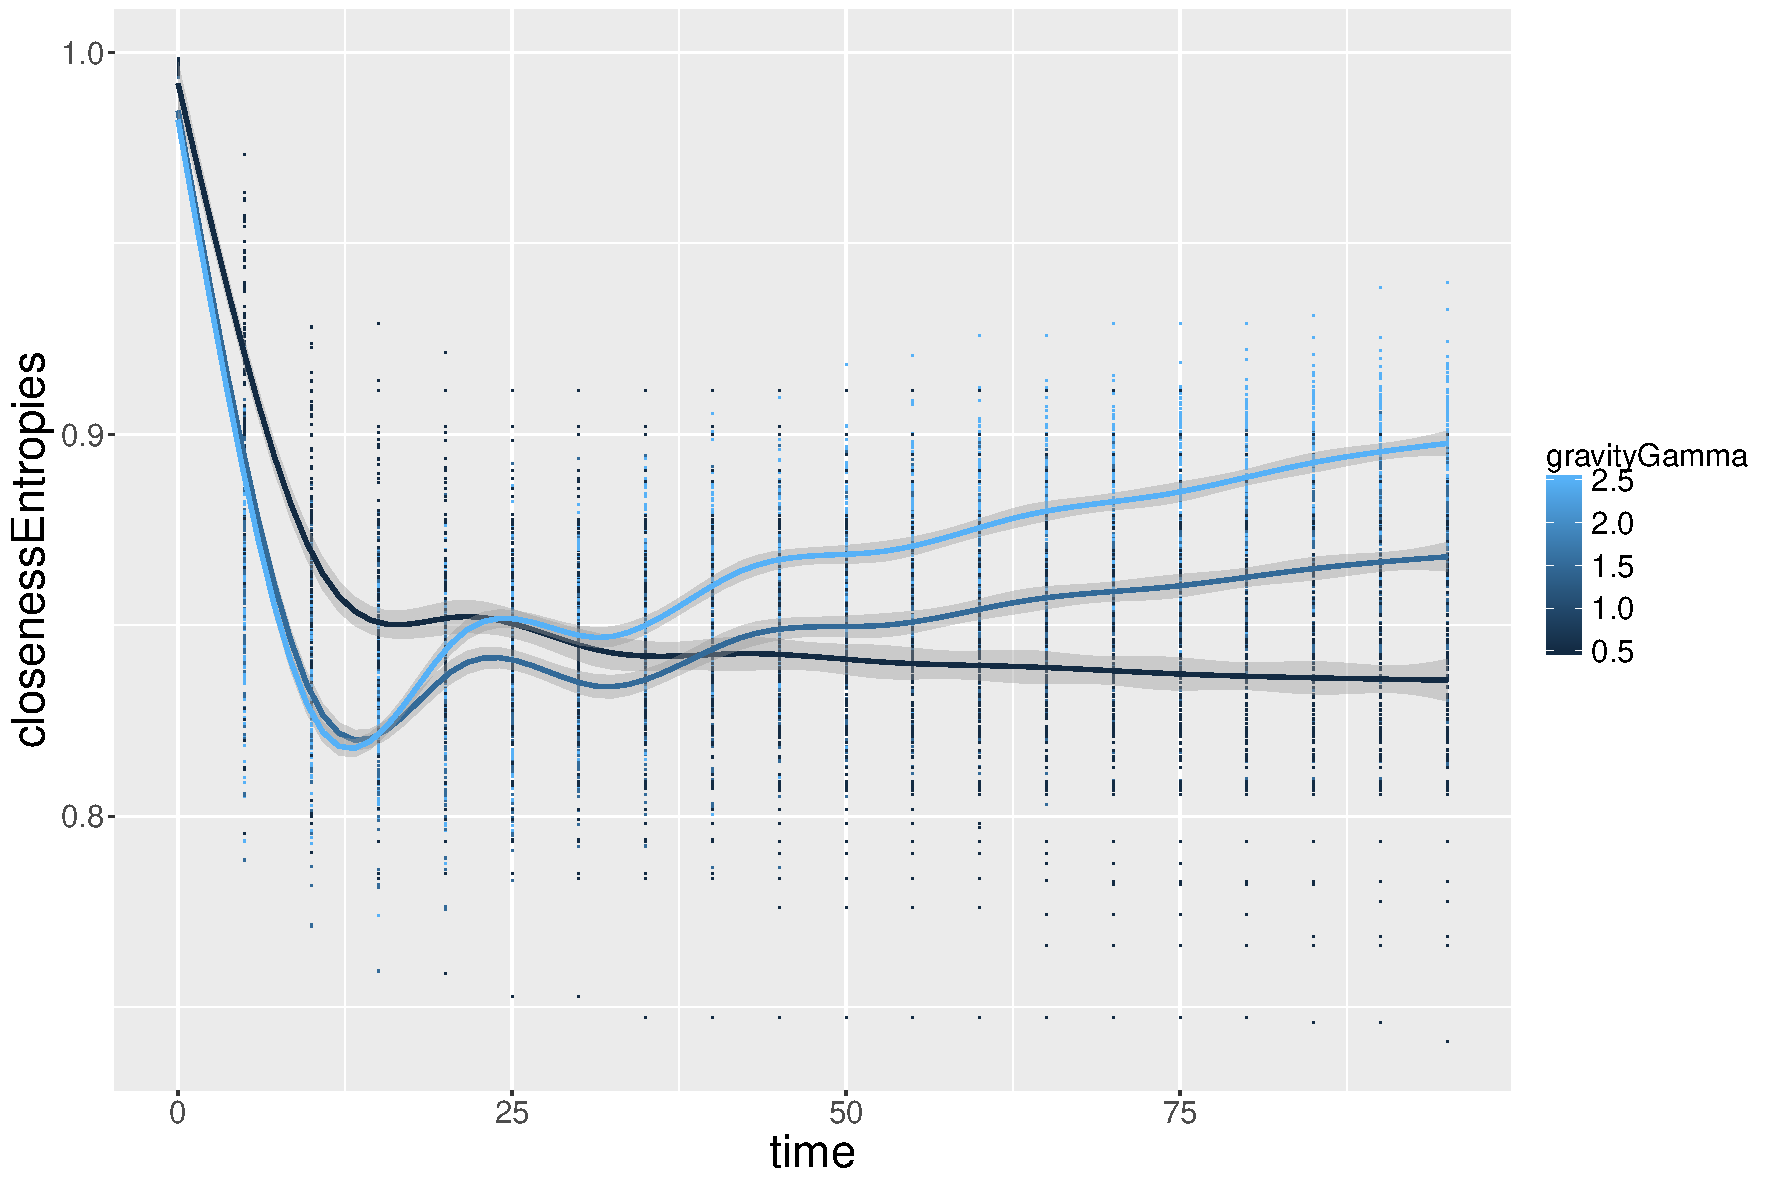
\includegraphics[width=0.48\linewidth]{Figures/MacroCoEvolExplo/closenessEntropies_networkGamma2.5_networkSpeed110_gravityDecay0.016_networkThreshold11.pdf}
	%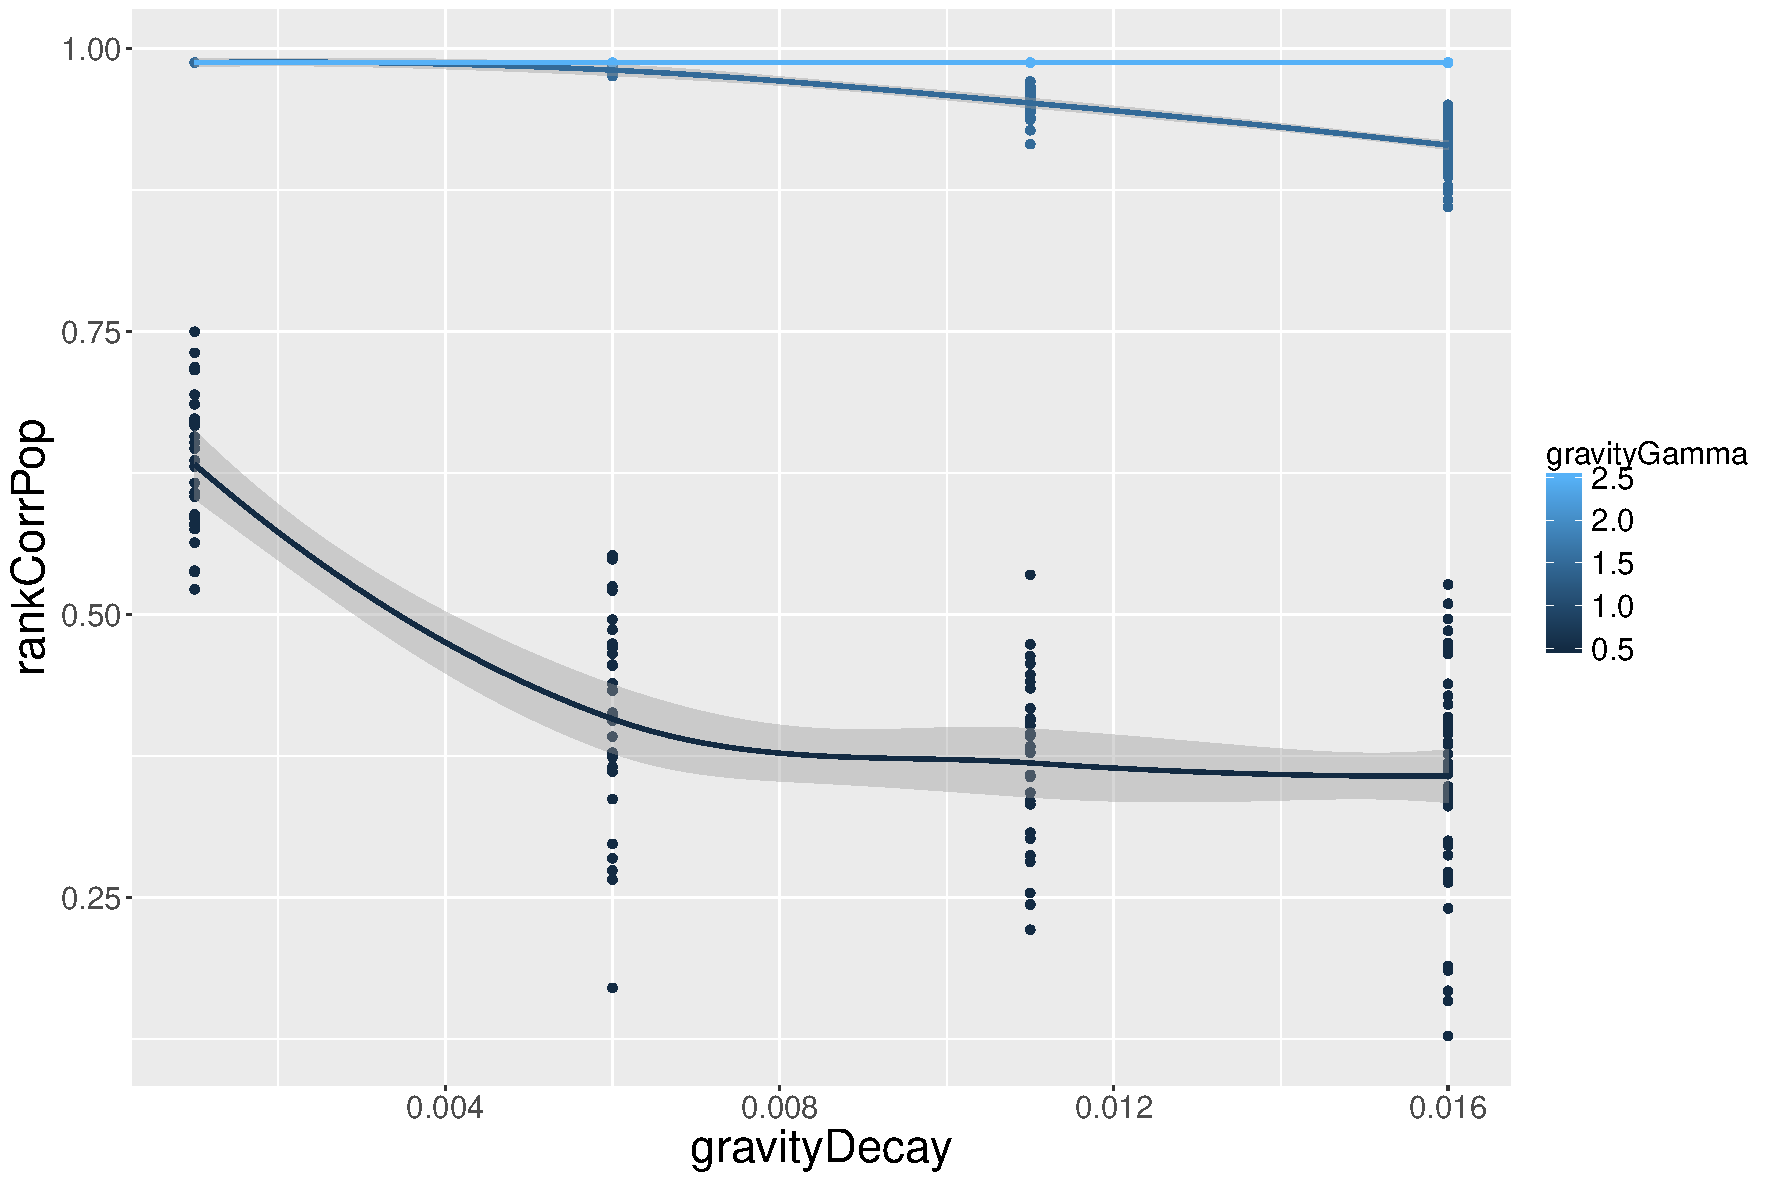
\includegraphics[width=0.48\linewidth]{Figures/MacroCoEvolExplo/rankCorrPop_networkSpeed110_networkThreshold11_networkGamma2.5.pdf}\\
	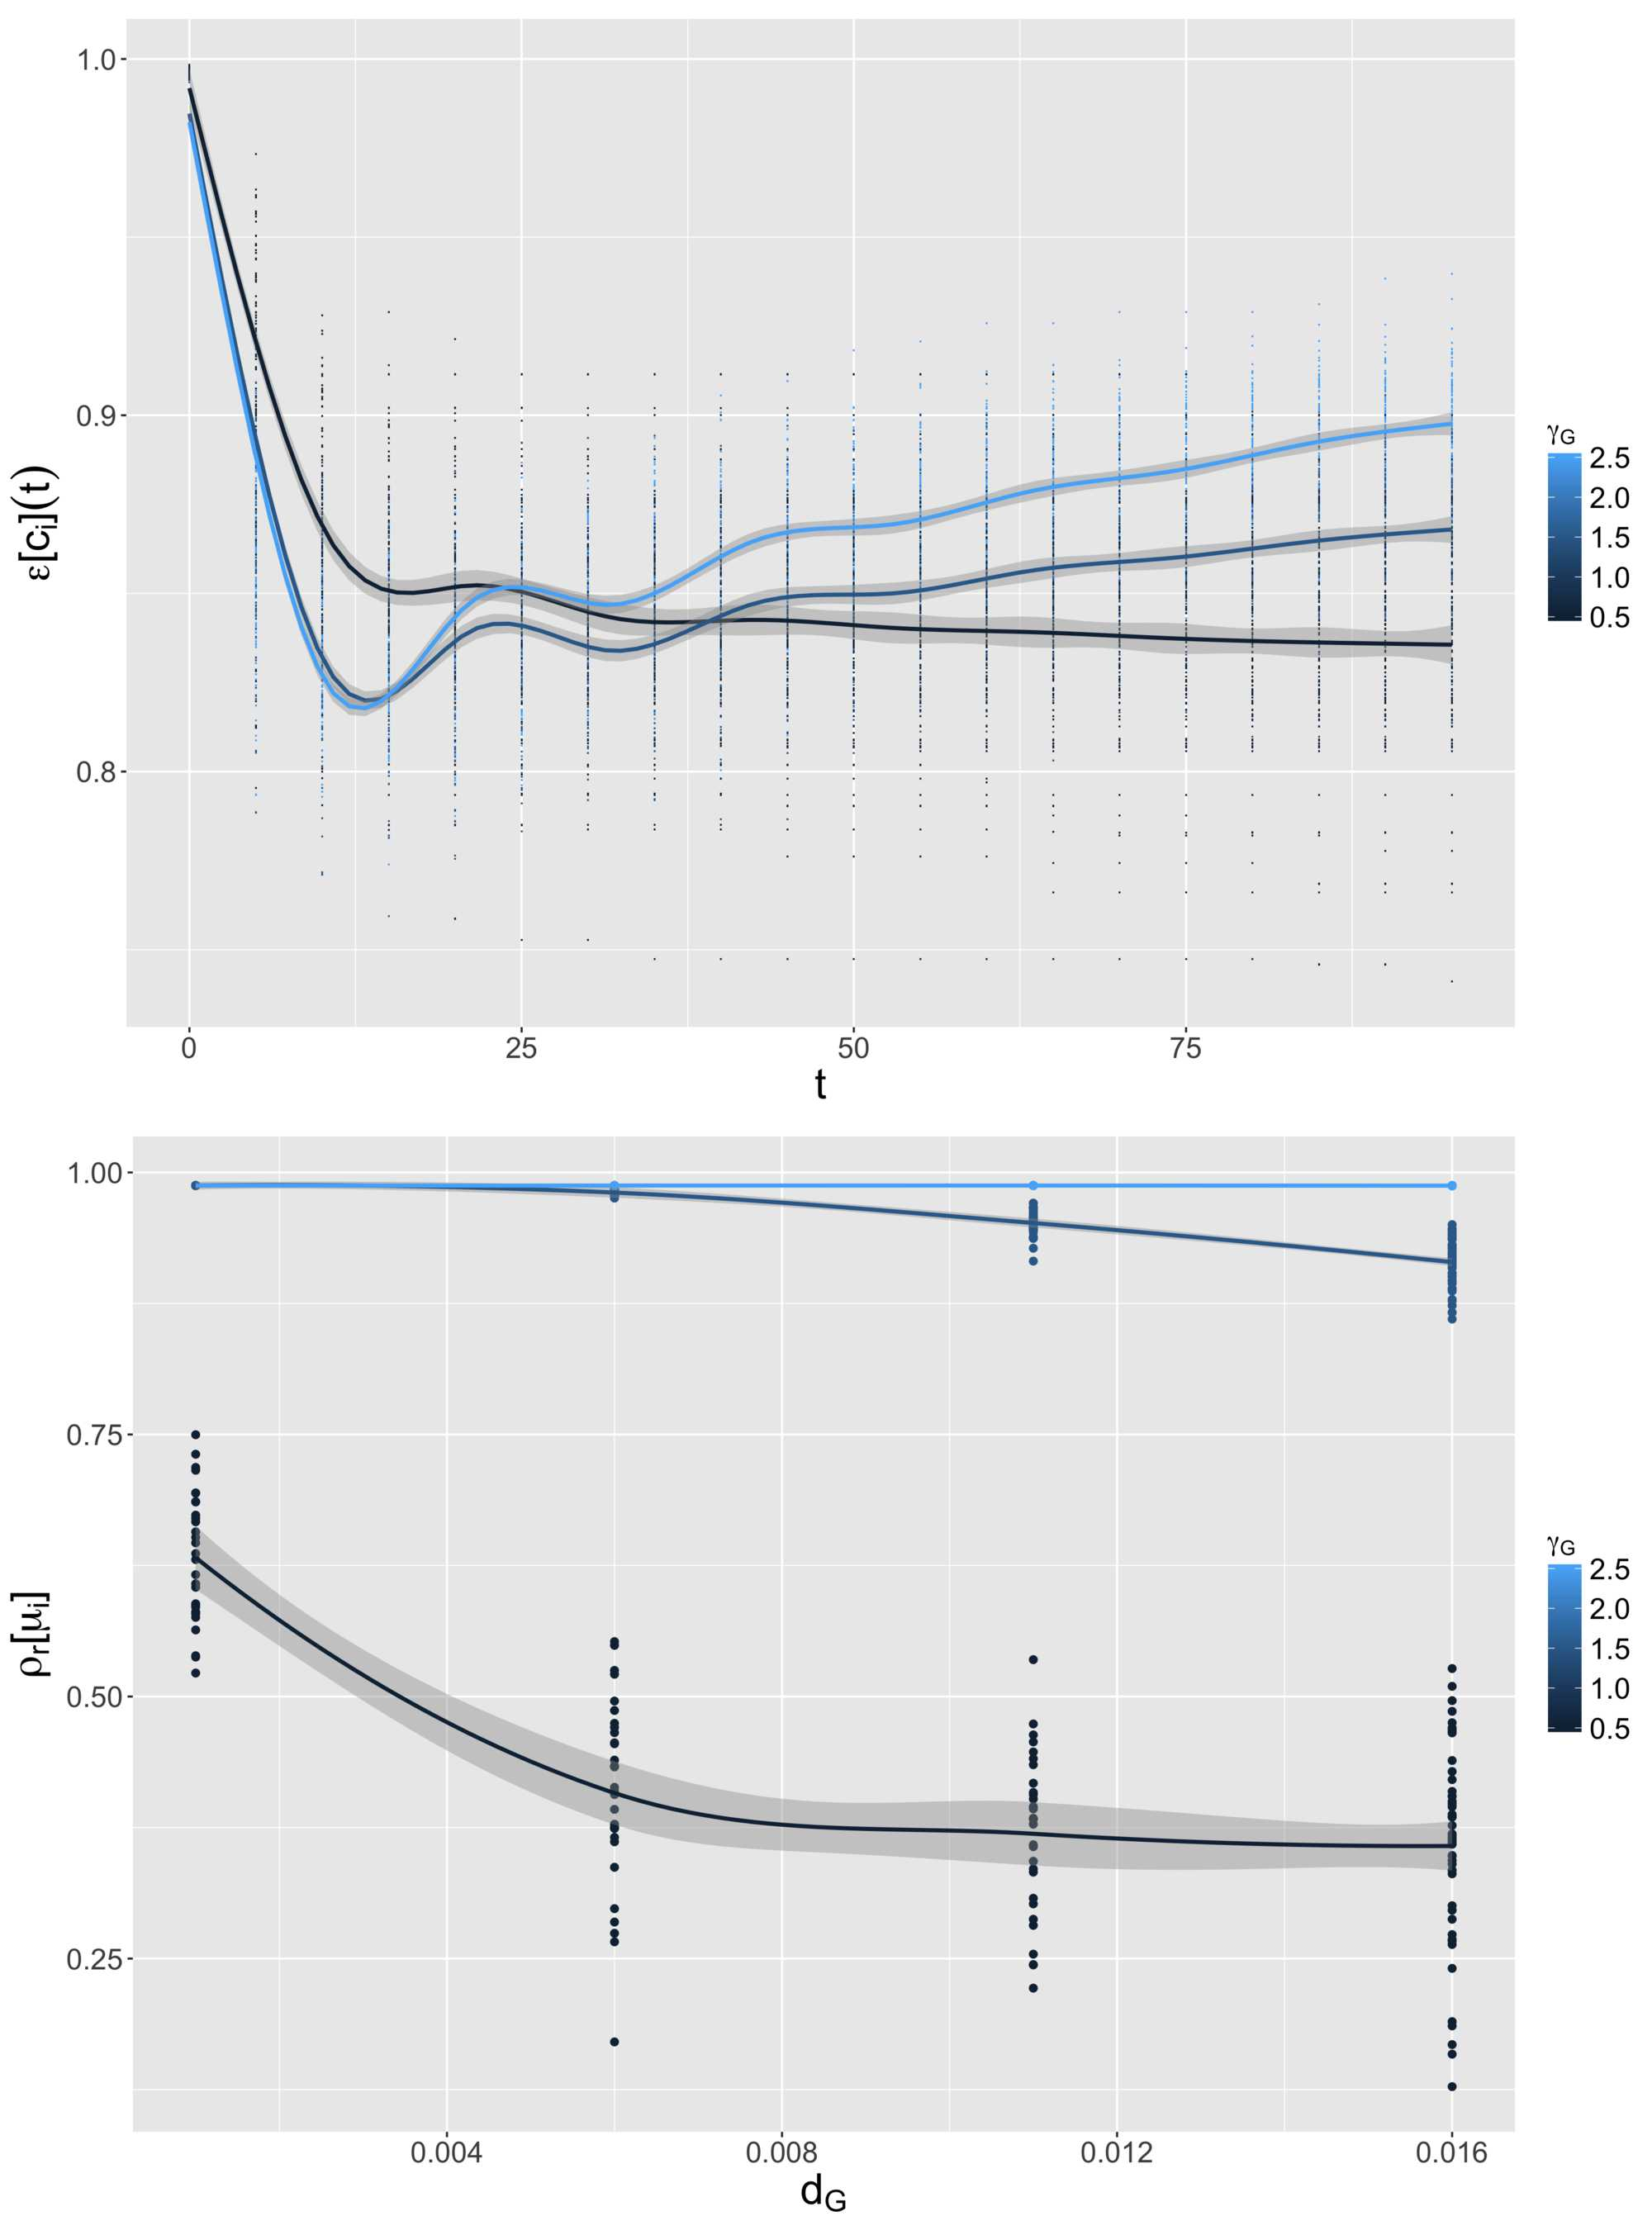
\includegraphics[width=\linewidth,height=0.85\textheight]{Figures/Final/6-1-3-fig-macrocoevolexplo-behavior.jpg}
	\caption[Model Behavior][Comportement du modèle SimpopNet]{\textbf{Model behavior for the spatial configuration $N_S=80,\alpha_S=0.5,d_S=10,n_S=30$.}\label{fig:macrocoevolexplo:behavior}}{\textbf{Comportement du modèle pour la configuration spatiale $N_S=80,\alpha_S=0.5,d_S=10,n_S=30$.} \textit{(Haut)} Trajectoires temporelles de l'entropie des centralités de proximité, pour $\gamma_N = 2.5$, $v_0 = 110$, $d_G = 0.016$, $\theta_N = 11$, en fonction de $\gamma_G$ (couleur); \textit{(Bas)} Corrélation de rang pour la population, en fonction de $d_G$ et de $\gamma_G$ (couleur), pour $\theta_N = 11$, $\gamma_N = 2.5$.\label{fig:macrocoevolexplo:behavior}}
\end{figure}
%%%%%%%%%%%%%%%%



Le comportement des indicateurs de corrélation est montré en Fig.~\ref{fig:macrocoevolexplo:correlations}. Concernant l'effet de la distance sur les corrélations entre variables, c'est-à-dire l'évolution de $\rho_d$, il est intéressant de noter que l'augmentation de $d_G$ diminue systématiquement les niveaux de corrélation, ce qui correspond à la complexification mise en valeur précédemment. Comme attendu, $\rho_d\left[d\right]$ décroit en fonction de la distance, et des valeurs non nulles pour la corrélation entre population et centralité pour une forte hiérarchie $\gamma_G$, ce qui montre que les régimes d'adaptation simultanée sont rares dans ce modèle.

\subsubsection{Causality regimes}{Régimes de causalité}

Enfin, en étudiant $\rho_{\tau}$ (Fig.~\ref{fig:macrocoevolexplo:correlations}, panneau du bas), nous constatons que les régimes de causalité au sens de~\ref{sec:causalityregimes}, ne sont pas très variés (comme le confirme la Fig.~\ref{fig:app:macrocoevolexplo:laggedcorrs} en Annexe~\ref{app:sec:macrocoevolexplo} pour une plage plus large de paramètres). La population est systématiquement causée par la centralité, mais il n'existe pas de régime où l'on observe le contraire. Il s'agit d'une logique d'effet de renforcement de la hiérarchie par la centralité, mais pas d'une configuration avec causalités circulaires, et donc pas d'une une co-évolution à proprement parler comme nous l'avons définie au sens statistique.




% -- positive only
%unique(signs$sign)
%[1] "00/00/00" "00/00/10" "01/00/10" "00/10/00" "01/00/00"


%  -- with negative --
% unique(signs$sign)
% [1] "-1-1/00/00"     "-1-1/00/-10"    "-1-1/00/10"     "-10/00/00"      "-10/00/10"      "01/00/10"      
% [7] "00/00/10"       "-11/00/10"      "-1-1/-10/-10"   "-1-1/-1-1/-10"  "-1-1/-10/-1-1"  "-1-1/-1-1/-1-1"
% [13] "-1-1/10/-10"    "-1-1/-1-1/00"   "00/00/00"       "0-1/00/00"      "01/00/00"       "-1-1/-10/00"   
% [19] "01/00/-10"      "-1-1/1-1/-10" 



%%%%%%%%%%%%%%%%
\begin{figure}
	%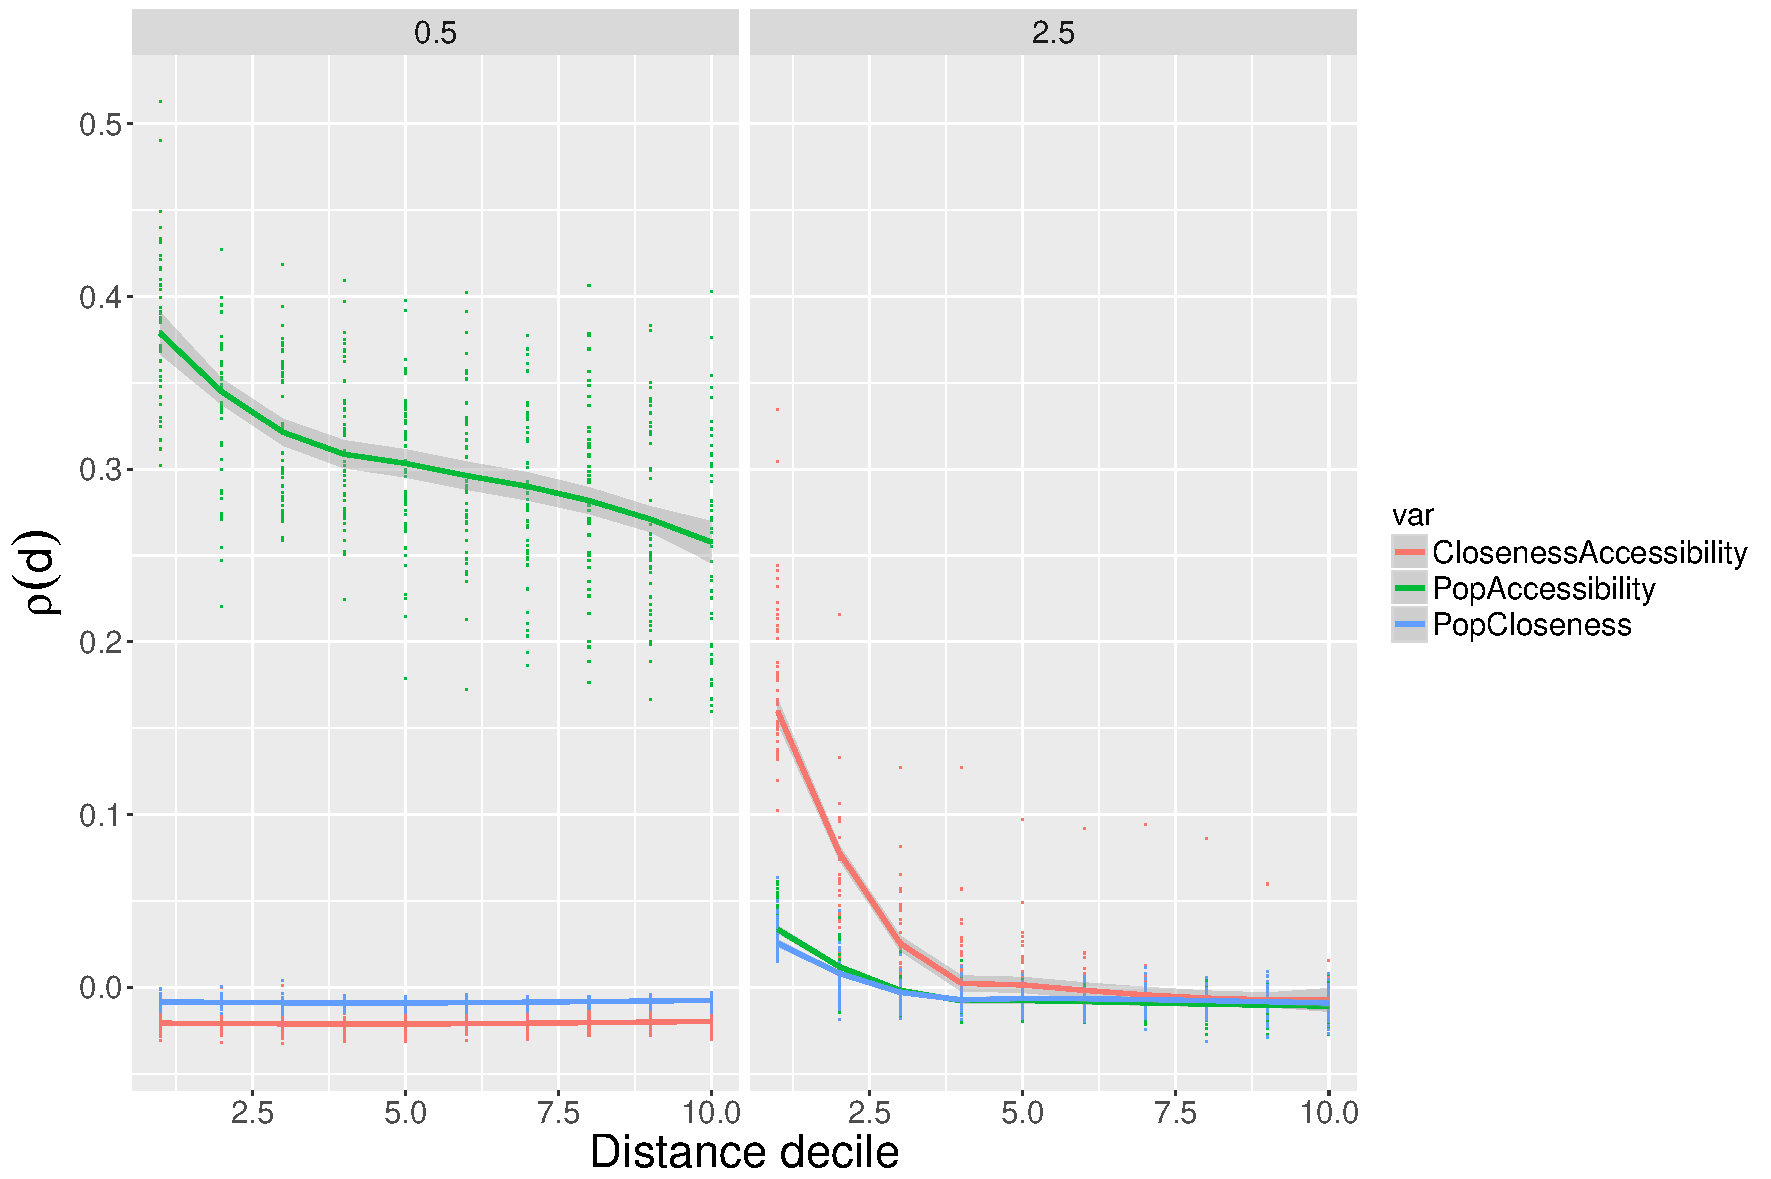
\includegraphics[width=0.48\linewidth]{Figures/MacroCoEvolExplo/distcorrs_networkGamma2.5_networkSpeed110_gravityDecay0.016_networkThreshold11.pdf}
	%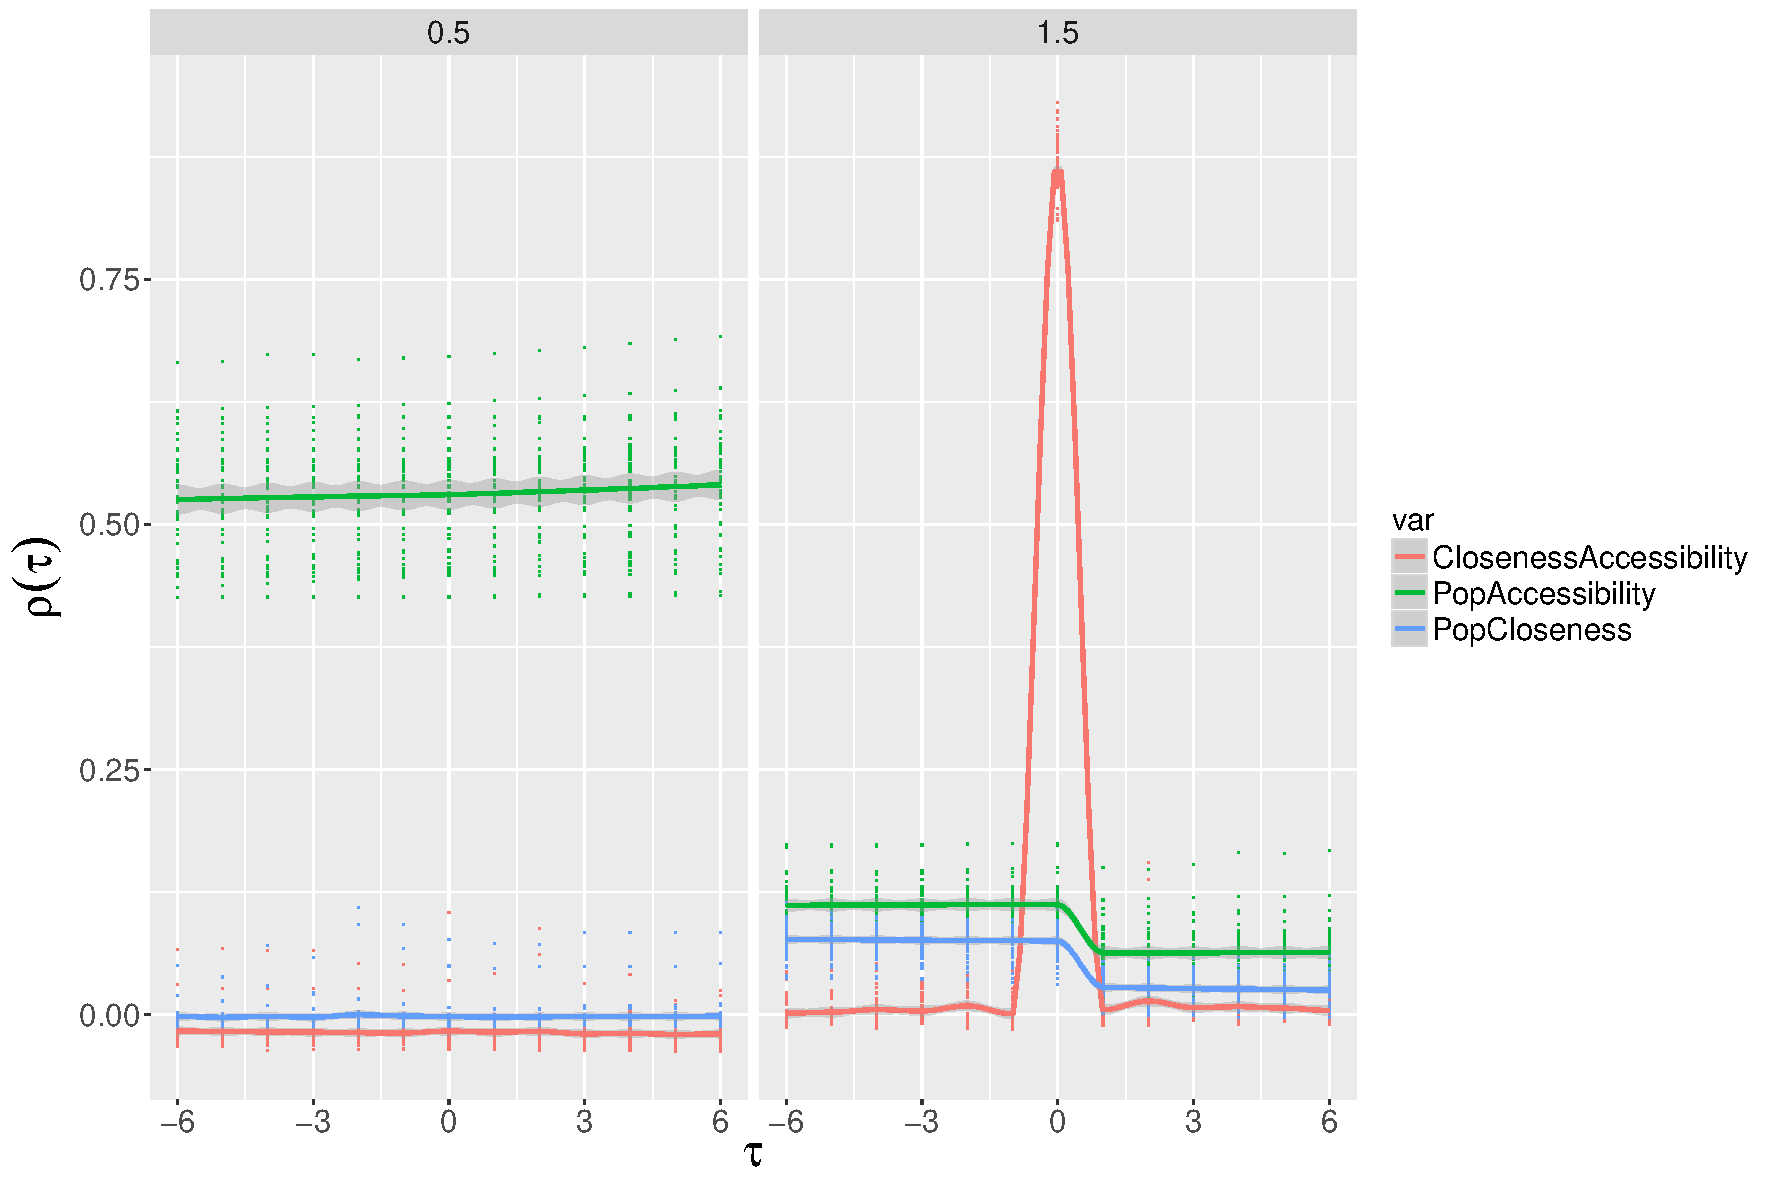
\includegraphics[width=0.48\linewidth]{Figures/MacroCoEvolExplo/laggedcorrs_networkGamma2.5_networkSpeed10_gravityDecay0.016_networkThreshold21.pdf}
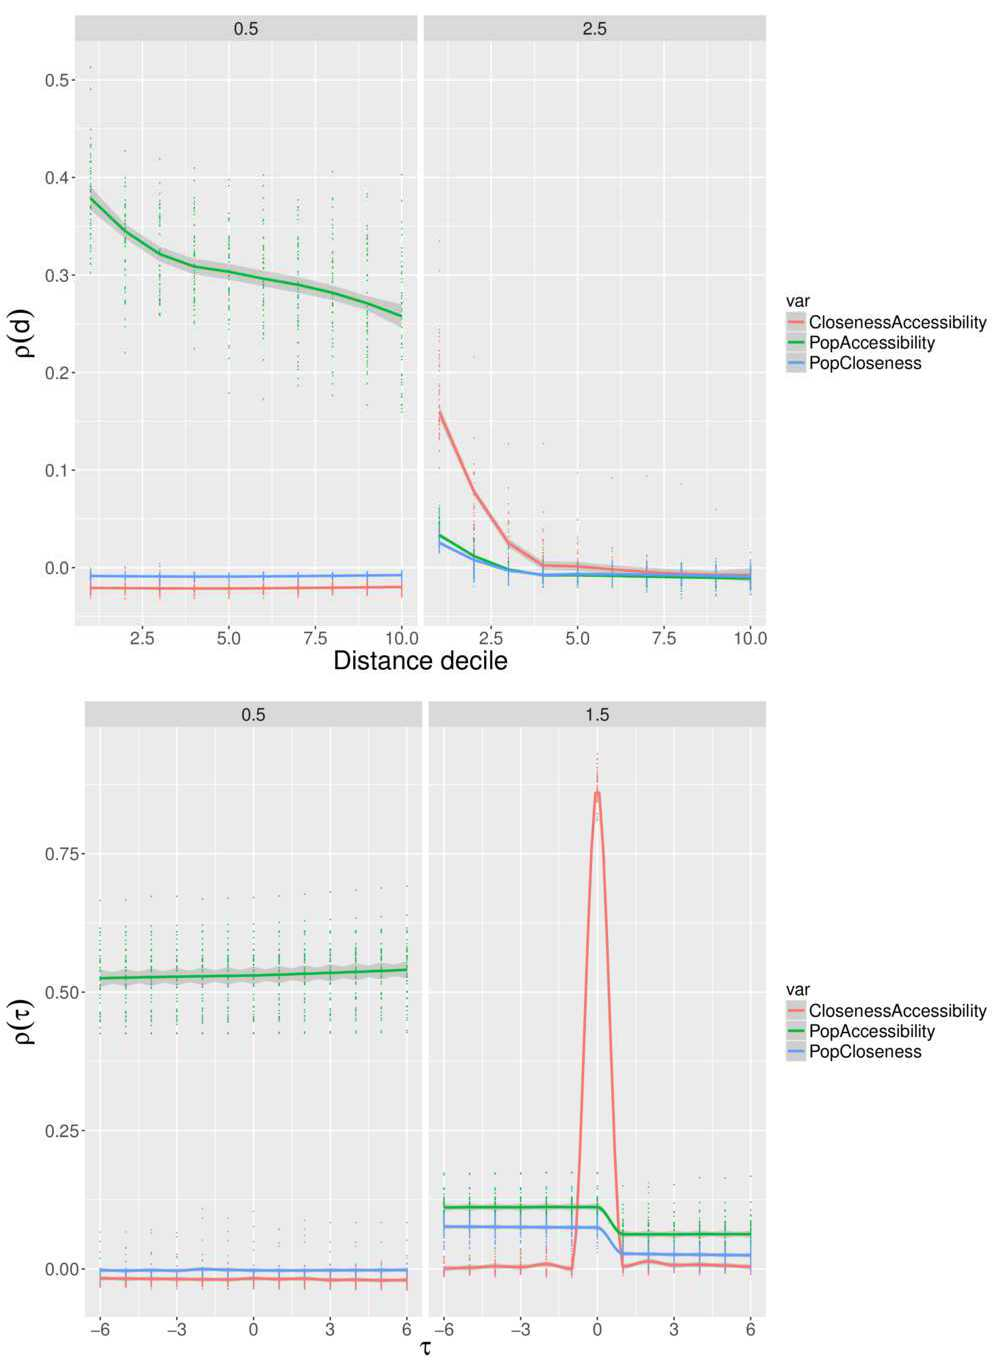
\includegraphics[width=\linewidth,height=0.9\textheight]{Figures/Final/6-1-3-fig-macrocoevolexplo-correlations.jpg}
	\caption[Correlations][Motifs de corrélations dans l'espace et le temps]{\textbf{Correlations in the model for the spatial configuration $N_S=80,\alpha_S=0.5,d_S=10,n_S=30$.}\label{fig:macrocoevolexplo:correlations}}{\textbf{Corrélations dans le modèle pour la configuration spatiale $N_S=80,\alpha_S=0.5,d_S=10,n_S=30$.} \textit{(Haut)} Corrélations en fonction de la distance, pour les couples de variables (couleur), pour $\gamma_N = 2.5$, $\theta_N = 21$, $v_0 = 10$, et pour $d_G$ (colonnes) et $\gamma_G$ (lignes) variables ; \textit{(Bas)} Corrélations retardées pour les mêmes paramètres.\label{fig:macrocoevolexplo:correlations}}
\end{figure}
%%%%%%%%%%%%%%%%


Cette exploration brève nous permet d'affirmer que ce modèle capture des trajectoires urbaines d'une certaine complexité, mais qu'il ne reproduit apparemment pas de régimes de co-évolution.




\stars

Nous avons ainsi dans cette section introduit les outils pour comprendre les trajectoires produites par un modèle de co-évolution, et testé ceux-ci sur le modèle SimpopNet.

Par la suite, nous explorerons dans le même esprit une extension co-évolutive du modèle d'interaction développé en~\ref{sec:interactiongibrat}, et chercherons à établir dans quelle mesure il est capable de capturer des dynamiques co-évolutives.



\stars








